\section{Results and Discussion}

\subsection{Standard Evolutionary Experiments}

\begin{figure}%[!htbp]

\begin{center}
\setlength\tabcolsep{1.5pt} % default value: 6pt
\medmuskip=-2mu
\thinmuskip=-2mu
\thickmuskip=-2mu
\nulldelimiterspace=-1pt
\scriptspace=0pt
\begin{tabular}{ | c || c c c | c c c | }
  \multicolumn{1}{c}{} & \multicolumn{3}{c}{Competitors} & \multicolumn{3}{c}{Mean Dominant ($\pm S.D.$)} \\
 \cline{2-7}
  \multicolumn{1}{c|}{} & \tiny{$P_{1} = 1.0$} & \tiny{$P_{2} = P_{1}$} & \tiny{$P_{2} > P_{1}$} & \tiny{$P_{1} = 1.0$} & \tiny{$1.0 > P_{1} > P_{2}$} & \tiny{$P_{2} \geq P_{1}$}  \\
 \hline
 $n$ & 1 & 1 & 1 & 9 & 7 & 34  \\
 \hhline{|=||===|===|}
 $A_1$ & 0.00 & 1.00 & 1.00 & $0.23 \pm 0.35$ & $0.50 \pm 0.47$ & $0.57 \pm 0.46$ \\
 $A_2$ & 1.00 & 0.91 & 1.00 & $1.00 \pm  0.00$ & $1.00 \pm 0.00$ & $1.00 \pm 0.00$ \\
 \hline
 $P_{c}$ & 0.85 & 0.00 & 0.00 & $0.00 \pm 0.00$ & $0.00 \pm 0.00$ & $0.03 \pm 0.05$ \\
 $P_1$ & 0.07 & 1.00 & 0.00 & $1.00 \pm 0.00$ & $0.60 \pm 0.07$ & $0.28 \pm 0.16$ \\
 $P_2$ & 0.08 & 0.00 & 1.00 & $0.00 \pm 0.00$ & $0.40 \pm 007$ & $0.69 \pm 0.14$ \\
 \hline
 $C_1$ & 21.8 & 7.2 & 9.9 & $3.90 \pm 0.60$ & $3.38 \pm 0.33$ & $3.03 \pm 0.69$ \\
 $C_2$ & 101.2 & 274.2 & 238.2 & $230.6 \pm 71.1$ & $192.7 \pm 45.3$ & $271.6 \pm 73.6 $ \\
 \hline
 $E_{c}$ & 0.21 & 0.00 & 0.00 & $0.29 \pm 0.37$ & $0.44 \pm 0.59$ & $0.21 \pm 0.75$ \\
 $E_1$ & 1.21 & 30.1 & 0.00 & $47.2 \pm 21.7$ & $21.3 \pm 12.0$ & $4.62 \pm 7.05$ \\
 $E_2$ & 2.49 & 54.1 & 38.8 & $231.2 \pm 94.3$ & $283.1 \pm 57.0$ & $325.4 \pm 68.9$ \\
 \hline
 $M_{c}$ & 0.53 & 0.30 & 0.90 & $0.33 \pm 0.41$ & $0.74 \pm 0.31$ & $0.67 \pm 0.35$ \\
 $M_1$ & 1.00 & 0.00 & 1.00 & $0.52 \pm 0.41$ & $0.65 \pm 0.46$ & $0.68 \pm 0.38$ \\
 $M_2$ & 0.00 & 1.00 & 0.24 & $0.45 \pm 0.39$ & $0.52 \pm 0.37$ & $0.50 \pm 0.42$ \\
 \hline
 $S_1$ & 0.56 & 1.00 & 0.68 & $0.65 \pm 0.38$ & $0.55 \pm 0.40$ & $0.47 \pm 0.42$ \\
 $S_2$ & 1.00 & 0.84 & 0.71 & $0.51 \pm 0.43$ & $0.35 \pm 0.39$ & $0.45 \pm 0.39$ \\
 \hline
\end{tabular}
\end{center}
\caption{
Enumerations for genotypes used as seeds for competition experiments (left) and enumerations for mean values of the most abundant genotype at the end of evolutionary runs (right), both sorted by resource-caching strategy.
}
\label{fig:genotypes}
\end{figure}


\begin{figure}[t]
\begin{center}
\begin{subfigure}[b]{0.82\columnwidth}
  \includegraphics[width=\columnwidth,trim={2.5cm 0.5cm 2.5cm 1cm},clip]{img/ChannelMap_1022_update19500000}
  \caption{Mean $P_0 = 0.77$, $P_1 = 0.089$, $P_2 = 0.14$; generation 20,475}
  \label{fig:ChannelMap_1022}
\end{subfigure}

\begin{subfigure}[b]{0.82\columnwidth}
  \includegraphics[width=\columnwidth,trim={2.5cm 0.5cm 2.5cm 1cm},clip]{img/ChannelMap_1041_update19500000}
  \caption{Mean $P_1 = 1.0$; generation 23,971}
  \label{fig:ChannelMap_1041}
\end{subfigure}

\begin{subfigure}[b]{0.82\columnwidth}
  \includegraphics[width=\columnwidth,trim={2.5cm 0.5cm 2.5cm 1cm},clip]{img/ChannelMap_1008_update19500000}
  \caption{Mean $P_2 = 1.0$; generation 25,841}
  \label{fig:ChannelMap_1008}
\end{subfigure}

\caption{
State of same-channel zero- and one-level signaling networks after $19.5$ million updates of evolution with different population mean $P_0$, $P_1$, and $P_2$.
Zero-level channels coded by HSV value are separated by white borders and one-level channels coded by HSV hue are separated by black borders.
}
\label{fig:outcome_grids}
\end{center}
\end{figure}


\begin{figure}[t]
\begin{center}
\begin{subfigure}[b]{0.5\columnwidth}
  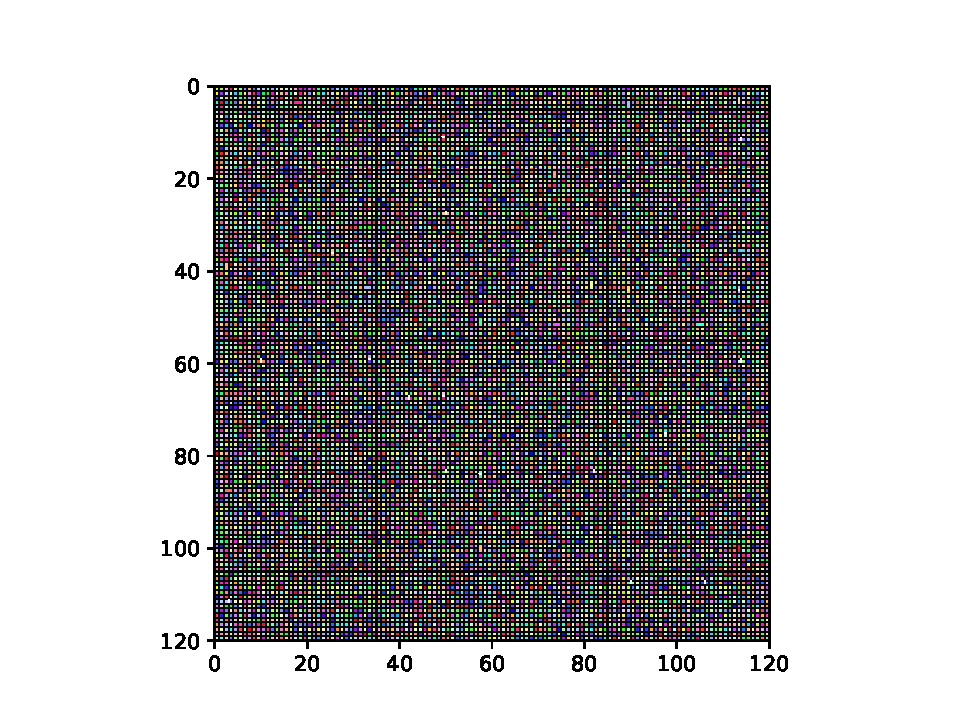
\includegraphics[width=\columnwidth,trim={2.5cm 0.5cm 2.5cm 1cm},clip]{img/ChannelMap_1011_update0}
  \caption{Update 0 (Generation 0)}
  \label{fig:ChannelMap_1011_update0}
\end{subfigure}%
\begin{subfigure}[b]{0.5\columnwidth}
  \includegraphics[width=\columnwidth,trim={2.5cm 0.5cm 2.5cm 1cm},clip]{img/ChannelMap_1011_update1000000}
  \caption{Update 1 million (Generation 927)}
  \label{fig:ChannelMap_1011_update1000000}
\end{subfigure}
\begin{subfigure}[b]{0.5\columnwidth}
  \includegraphics[width=\columnwidth,trim={2.5cm 0.5cm 2.5cm 1cm},clip]{img/ChannelMap_1011_update2000000}
  \caption{Update 2 million (Generation 1917)}
  \label{fig:ChannelMap_1011_update2000000}
\end{subfigure}%
\begin{subfigure}[b]{0.5\columnwidth}
  \includegraphics[width=\columnwidth,trim={2.5cm 0.5cm 2.5cm 1cm},clip]{img/ChannelMap_1011_update4000000}
  \caption{Update 4 million (Generation 4053)}
  \label{fig:ChannelMap_1011_update4000000}
\end{subfigure}
\begin{subfigure}[b]{0.5\columnwidth}
  \includegraphics[width=\columnwidth,trim={2.5cm 0.5cm 2.5cm 1cm},clip]{img/ChannelMap_1011_update5000000}
  \caption{Update 5 million (Generation 5173)}
  \label{fig:ChannelMap_1011_update5000000}
\end{subfigure}%
\begin{subfigure}[b]{0.5\columnwidth}
  \includegraphics[width=\columnwidth,trim={2.5cm 0.5cm 2.5cm 1cm},clip]{img/ChannelMap_1011_update7000000}
  \caption{Update 7 million (Generation 7312)}
  \label{fig:ChannelMap_1011_update7000000}
\end{subfigure}
\caption{
Progression of of same-channel level-zero and level-one signaling networks states in an evolutionary run where population mean $P_1 > P_{self}, P_0$ evolved.
Level-zero channels coded by HSV value are separated by white borders and level-one channels coded by HSV hue are separated by black borders.
}
\label{fig:grid_progression}
\end{center}
\end{figure}


A spectrum of resource allocation strategies ranging from purely allocation to level-one same-channel resource pools to primarily allocation to level-two same-channel resource pools were observed at the conclusion of different runs of our evolutionary simulation (mean cellular generation 37,168 with standard deviation 4,684).
We interpret these outcomes as ranging between individuality at the level of first-level same-channel groups to individuality at the level of second-level same-channel groups.
Figure \ref{fig:outcome_grids} shows the level-one and level-two signaling networks at the end of runs where first-, split-, and second-level resource allocation evolved, respectively.
First-level allocators form somewhat irregular level-two amalgamations of diverse level-one networks.
Second-level allocators form highly regular diamond-shaped level-two signaling networks.
Split-allocation individuals exhibit a level-two phenotype of intermediate regularity.
Figure \ref{fig:grid_progression} shows a time series of signaling network snapshots in an evolutionary run where second-level individuality evolved.

Table \ref{table:genotypes} summarizes most-common genotypes observed at the end of our evolutionary simulations.
In the standard treatment, all evolved genotypes had $A_2$ fixed at $1.0$.
So, reproduction over cells sharing the same level-two channel was universally avoided;
genotypes evolved so that cells declined to reproduce when they were located at the interior of level-two same-channel signaling networks.

However, a variety of resource-caching strategies evolved.
Most-abundant genotypes at the end of nine evolutionary runs exclusively cached resource in organisms' level-one signaling network's pool (i.e., $P_1 = 1.0$).
We observed strategies where resource was primarily, but not entirely, cached in an organism's level-one signaling network pool (i.e., $1.0 > P_1 > P_2$) as the most-abundant genotype at the end of seven evolutionary runs.
In one run, the most-abundant final genotype split resources evenly between an organism's level-one and level-two signaling network pool ($P_1 = P_2 = 0.5$).
Finally, we observed strategies where resource was primarily, but not entirely, cached in an organism's level-two signaling network pool (i.e., $1.0 > P_2 > P_1$) as the most-abundant genotype at the end of 33 evolutionary runs.

We suspect that a trade-off between growth rate and long-term stability prompted the universal allocation of at least some resource to level-one pools and/or cell stockpiles.
Cell- and level-one resource caching might function something like saving for a rainy day.
Because reproduction over level-two channel-mates was universally avoided, cells and level-one same-channel networks situated at the interior of a larger level-two same-channel network do not expend their resource pools unless that larger level-two same-channel network is damaged, exposing them to directly-adjacent cells of a different level-two channel.
Thus, resource accumulates in cell stockpiles and level-one pools until the level-two same-channel network comes under stress.
Split allocation might also represent hedging against defection of a second-level channel-mate by via somatic mutation.

Indeed, we did observe selection for apoptosis in the 41 replicates where the dominant genotype employed second-level resource caching.
In these replicates, the average population mean value of $M_{c}$ was 0.68 with standard deviation 0.33, significantly greater than the value $M_{c} = 0.5$ we would expect in the absence of a selective pressure on apoptosis response to mutation ($p < 0.001$, bootstrap test).

\begin{figure}[t]
\begin{center}

\begin{subfigure}[b]{\columnwidth}
  \includegraphics[width=\columnwidth]{img/champion_res_pool1_vs_champion_damage_suicide0}
  \label{fig:champion_res_pool1_vs_champion_damage_suicide0}
\end{subfigure}

\begin{subfigure}[b]{\columnwidth}
  \includegraphics[width=\columnwidth]{img/champion_res_pool2_vs_champion_damage_suicide0}
  \label{fig:champion_res_pool2_vs_champion_damage_suicide0}
\end{subfigure}

\caption{
TODO
}
\label{fig:damage_suicide}
\end{center}
\end{figure}


To assess whether heavy second-level resource allocators, which we characterize as higher-level individuals, were more likely to employ apoptosis to mitigate somatic mutation, we examined the relationship between first- and second-level resource pooling and cellular apoptosis at the conclusion of our 50 replicate evolutionary trials.
We observed a significant negative correlation between dominant genotype $P_1$ and $M_{c}$ ($p < 0.05$; bootstrap test; Figure \ref{fig:champion_res_pool1_vs_champion_damage_suicide0}) and a significant positive correlation between dominant genotype $P_2$ and $M_{c}$ ($p < 0.05$; bootstrap test; Figure \ref{fig:champion_res_pool2_vs_champion_damage_suicide0}).
This result suggests that second-level individuals, in particular, relied on apoptosis to mitigate somatic mutation.

We also assessed whether higher-level individuals provided larger resource endowments to their second-level propagules (offspring sharing neither the level-one nor the level-two channel ID with the parent).
We examined the relationship between first and second-level resource pooling and dominant genotype second-level propagule endowment at the conclusion of our 50 replicate evolutionary trials.
We observed a significant negative correlation between dominant genotype $P_1$ and $E_2$ ($p < 0.05$; bootstrap test) and a significant positive correlation between dominant genotype $P_2$ and $E_2$ ($p <  0.05$; bootstrap test).
Second-level individuals might provide larger endowments to propagules simply due to a greater capacity to collect resource or perhaps because of stronger selection for well-endowed offspring when competing against other second-level individuals.

This result prompts the reverse question: do lower-level individuals provide  larger resource endowments to first-level propagules (offspring that do not share level-one channel ID with the parent but may or may not share level-two channel ID with the parent)?
Indeed, we observed a significant positive correlation between first-level resource sharing and first-level endowment ($p < 0.0001$; bootstrap test) and a significant negative correlation between second-level resource sharing and first-level endowment ($p < 0.0001$; bootstrap test).
Cells that pool resource with their smaller level-one same-channel group tend to invest more heavily into the direct offshoots of their level-one same-channel group than cells that pool resource with their larger level-two same-channel group.
This observation suggests that, although cells do not directly displace their level-one channel-mates, competitive dynamics between may be at play.

\subsection{Competition Experiments}

\begin{figure*}%[!htbp]
\begin{center}


\begin{subfigure}[b]{0.9\columnwidth}
  \includegraphics[width=\columnwidth,trim={2.5cm 0.5cm 2.5cm 1cm},clip]{img/ChannelMap_1030_update0}
  \caption{Update 0; cell gen. 0}
  \label{fig:ChannelMap_1030_update0}
\end{subfigure}%
\begin{subfigure}[b]{0.9\columnwidth}
  \includegraphics[width=\columnwidth,trim={2.5cm 0.5cm 2.5cm 1cm},clip]{img/ChannelMap_1030_update5552}
  \caption{Update 5552; cell gen. 4}
  \label{fig:ChannelMap_1030_update55520}
\end{subfigure}

\begin{subfigure}[b]{0.9\columnwidth}
  \includegraphics[width=\columnwidth,trim={2.5cm 0.5cm 2.5cm 1cm},clip]{img/ChannelMap_1030_update11104}
  \caption{Update 1104; cell gen. 9}
  \label{fig:ChannelMap_1030_update277600}
\end{subfigure}%
\begin{subfigure}[b]{0.9\columnwidth}
  \includegraphics[width=\columnwidth,trim={2.5cm 0.5cm 2.5cm 1cm},clip]{img/ChannelMap_1030_update22208}
  \caption{Update 22208; cell gen. 32}
  \label{fig:ChannelMap_1030_update22208}
\end{subfigure}

\begin{subfigure}[b]{0.9\columnwidth}
  \includegraphics[width=\columnwidth,trim={2.5cm 0.5cm 2.5cm 1cm},clip]{img/ChannelMap_1030_update55520}
  \caption{Update 55520; cell gen. 107}
  \label{fig:ChannelMap_1030_update1000000}
\end{subfigure}%
\begin{subfigure}[b]{0.9\columnwidth}
  \includegraphics[width=\columnwidth,trim={2.5cm 0.5cm 2.5cm 1cm},clip]{img/ChannelMap_1030_update1500000}
  \caption{Update 1500000; cell gen. 3511}
  \label{fig:ChannelMap_1030_update1500000}
\end{subfigure}
\caption{
Progression of of same-channel level-one and level-two signaling networks states in an evolutionary run where level-two resource sharing evolved.
Level-one channels are coded by color saturation and level-two channels are coded by color hue.
A single cell-like organism occupies each grid tile except for black tiles, which are empty.
}
\label{fig:eco_progression}
\end{center}
\end{figure*}


Next, we wanted to compare first-, second-, and split-level allocators to determine which genotype was the most fit.
We ran competition experiments between dominant genotypes from evolutionary runs representative of each of these strategies.
To prevent further evolution, we disabled mutation for these experiments.
To represent first-level allocators, we selected randomly from the nine pure first-level allocator dominant genotypes we observed.
To represent the split-level allocators, we selected the single dominant genotype where resource was partitioned exactly evenly between first- and second-level channel pools.
To represent second-level allocators, we selected the dominant genotype with the largest second-level allocation proportion.
Table \ref{table:genotypes} enumerates the three representative genotypes used.
Figure \ref{fig:eco_progression} shows a time series of signaling network snapshots in a competition experiment run.
Colonies of each genotype can be seen to grow from each seed and then clash, ultimately yielding a population dominated by second-level allocators.

Indeed, the second-level resource caching strategy became most abundant in all 50 trials.
Across the 50 replicates, at update 1.5 million (cellular generation 3489 with standard deviation 40) the second-level resource caching strategy constituted $90.2 \%$, with standard deviation $3.8 \%$, of the competing population of cells.
In the absence of mutation, second-level allocators tend to exhibit greater fitness than split- and first-level allocators ($p < 0.0001$; two-tailed exact test).


\begin{figure}[!htbp]
\begin{center}

\begin{subfigure}[b]{0.5\columnwidth}
  \includegraphics[width=\columnwidth]{img/mean_res_pool1_vs_net_reproduction}
  \caption{
  Correlation plot of population mean $P_0$ and population net reproduction rate.
  }
  \label{fig:mean_res_pool1_vs_net_reproduction}
\end{subfigure}%
\begin{subfigure}[b]{0.5\columnwidth}
  \includegraphics[width=\columnwidth]{img/mean_res_pool2_vs_net_reproduction}
  \caption{
  Correlation plot of population mean $P_1$ and population net reproduction rate.
  }
  \label{fig:mean_res_pool2_vs_net_reproduction}
\end{subfigure}
\caption{
Mean resource caching strategies and net reproduction rate across populations.
A bootstrapped 95\% confidence interval for the fit is shaded.
}
\label{fig:net_reproduction}
\end{center}
\end{figure}


In competition experiments, however, higher-level individuals likely benefited from elimination of somatic mutation.
To assess the relative fitness of first- and second-level individuals without mutation disabled, we examined the relationship between first- and second-level resource pooling and the rate of cellular reproduction at the end of each of the 50 replicate evolutionary trials performed.
We observed a significant negative correlation between mean $P_1$ and cellular reproduction rate ($p < 0.0001$; bootstrap test; Figure \ref{fig:mean_res_pool1_vs_net_reproduction}) and a significant positive correlation between mean $P_2$ and cellular reproduction rate ($p < 0.0001$; bootstrap test; Figure \ref{fig:mean_res_pool2_vs_net_reproduction}).
This result suggests that second-level allocators tend to collect resource more effectively than split- and first-level allocators.

\subsection{Control Evolutionary Experiments}

\begin{figure}%[!htbp]
\begin{center}

\includegraphics[width=\columnwidth,trim={2.5cm 0.5cm 2.5cm 1cm},clip]{img/ChannelMap_1018_update3000000}

\caption{
End state (update 3000000, cell gen. 6916) of same-channel signaling networks evolved under the control treatment.
Level-one channels are coded by color saturation and level-two channels are coded by color hue.
A single cell-like organism occupies each grid tile except for black tiles, which are empty.
Level-one same-channel groups appear as uniformly-colored clumps, bounded by a white border.
Level-two same-channel groups appear as same-hue amalgamations of level-one groups, bounded by a black border.
}
\label{fig:outcome_control}
\end{center}
\end{figure}


Under control conditions where resource was distributed evenly to all cells regardless of same-channel group configuration, split-level resource caching also evolved.
Split-level allocation was the most common strategy at update 3 million in all replicates.
Strategies where resource was primarily, but not entirely, cached in an organism's level-one signaling network pool (i.e., $1.0 > P_1 > P_2$) were most-abundant at the end of 33 evolutionary runs and strategies where resource was primarily, but not entirely, cached in an organism's level-two signaling network pool (i.e., $1.0 > P_2 > P_1$) were most-abundant at the end of 17 evolutionary runs.
As shown in Table \ref{table:genotypes}, the average population mean of $P_1$ is greater in the control treatment than in the standard treatment at time-points matched by absolute elapsed update count and approximate elapsed cellular generations, but this difference is not statistically significant.

Consistent with the standard treatment, we observed strong selection against direct reproductive competition between channel-mates at update 3 million in the control treatment.
Nearly all most-common genotypes completely avoided reproducing over level-two channel-mates (i.e., $A_2 = 1.0$), except for a single most-common genotype where a very slim probability of reproducing over level-two channel-mates was allowed ($A_2 = 0.996$).

The emergence of resource-sharing and competition avoidance under control conditions suggests kin recognition alone can prompt some aspects of higher-level individuality.
However, we observed selection \textit{against} the apoptosis response to mutation, $M_{c}$, under control conditions.
Across 50 replicates of the control treatment, the average population mean value of $M_{c}$ was 0.18 with standard deviation 0.23 --- significantly less than the value $M_{c} = 0.5$ expected without selective pressure against apoptosis response to mutation ($p < 0.0001$, two-tailed t test).
Indeed, population mean $M_{c}$ for control runs was also significantly reduced compared to the standard treatment at time-points matched by absolute elapsed update count ($p < 0.001$; two-tailed t test) and by approximate elapsed cellular generations ($p < 0.001$; two-tailed t test).
Perhaps under control conditions, the apoptosis response to mutation is disfavored because kin groups stand to lose less from mutant members (i.e., the resource penalty for excessive same-channel network expansion is absent).
It appears that, at least in our system, kin recognition alone does not suffice to prompt full-fledged fraternal transitions in individuality.

In the absence of resource penalties for erroneous activation under control conditions, we also observed the evolution of larger same-channel groups.
At update 3 million, most-common genotypes encoded a level-two same-channel cap $C_2$ of 484.0 cells with standard deviation of 123.5.
Compared to the standard treatment, control runs exhibited larger mean level-two same-channel caps $C_2$ at time-points matched by absolute elapsed update count ($p < 0.0001$; two-tailed t test) and approximate elapsed cellular generations ($p < 0.0001$; two-tailed t test).
Even at 20 million updates, when evolution had elapsed around six times as many cellular generations in the standard treatment compared to the control treatment at update 3 million, mean level-two same-channel caps $C_2$ reached only 262.9 with standard deviation 72.2 under the standard treatment.
This is significantly smaller than mean $C_2$ under the control treatment at update 3 million ($p < 0.0001$; two-tailed t test).
Figure \ref{fig:outcome_control} depicts the comparatively large same-channel level two groups present at the end of a control run.
Table \ref{table:genotypes} summarizes most-common genotypes observed under the control treatment.
